\title{Concurrency and Parallel Programming \\ Assignment 6}
\author{David van Erkelens and Jelte Fennema \\ Department of Computer Science
    \\ University of Amsterdam} \date{\today}
\documentclass[12pt]{article}
\usepackage{graphicx}
\usepackage{color}
\begin{document}
\maketitle
\section{Wave}
\subsection{Comparison with sequential approach}
All problemsizes show a speedup when using the GPU. The smallest problemsize
only has a speedup of 1.7 and the largest speedup is 22.5 when using a
problemsize of 100000. All others have a speedup between 4 and 8, which is also
quite impressive.

\subsection{Comparing block sizes}
When the blocksizes are really small, 8 to 32 threads, the overhead is the main
factor that slows the program down. But when using reasonably sized blocks, the
difference in speed is quite marginal.

\subsection{Comparing accuracy}
Comparing accuracy isn't really possible when you don't know the correct answer.
What can be said though is that both implementations give different outcomes.
When comparing the result.txt that is generated by both, there are 4463
differences according to the utility diffstat. When comparing the two plots,
though a difference can't really be found using the naked eye.
By knowing a CPU has a lot of error checking components, it is more likely that
the CPU implumentation gives the moste accurate results. The differences are
only noticable when a really precise answer is needed.


\subsection{Graphs}
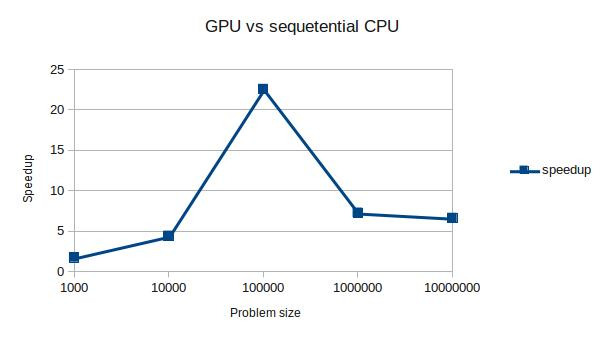
\includegraphics[width=\textwidth]{speedup.jpg}
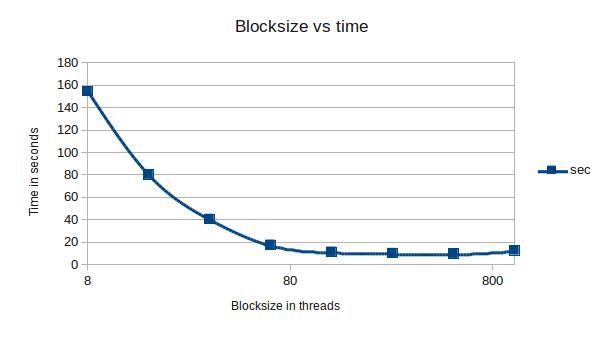
\includegraphics[width=\textwidth]{blocksize.jpg}



\section{Finding the maximum float in an array}
When comparing the times of the sequential approucht with the parallel approach
something strange was encountered. The time spent in the kernel when using the
parallel approach, actually calculating, was about 10 times smaller than the
time the sequential approach took. Only when adding the overhead from
allocating the memory on the graphical memory and copying the data to it, the
parallel approach took longer than the sequential approach.

This is probably, because the time the calculation costs is very low. The data
is only used once and has to be written back to the RAM afterards. When it came
to light that the memory access overhead was the main time consumer, some
timesavers in that area were looked into.

One was found. When the calculations finished, the whole array was copied back
to the RAM. This was not necessary, only the maximum value had to be copied.
This was changed in the next version and it performed slightly better, but on
avarage it was still slower than the sequential approach.



\end {document}
